% main.tex
\documentclass{report}
\usepackage{amsmath}
\usepackage{graphicx}
\graphicspath{{./figures/}}
\usepackage{subfigure}
\begin{document}
\chapter{Introduction}\label{ch:intro}
Hello
\section{Euler}\label{sec:euler}
\begin{equation}\label{eq:euler}
e^{i\pi}+1=0
\end{equation}
Equation~\eqref{eq:euler} is a beauty.

\begin{equation}\label{eq:einstein}
E = mc^2 \tag{*}
\end{equation}
Equation~\eqref{eq:einstein} is not bad either.

\begin{equation}\label{eq:gaslaw}
PV = nRT
\end{equation}
Equation~\eqref{eq:gaslaw} is a classic.

\begin{figure}[ht]
\centering
\subfigure[Union]{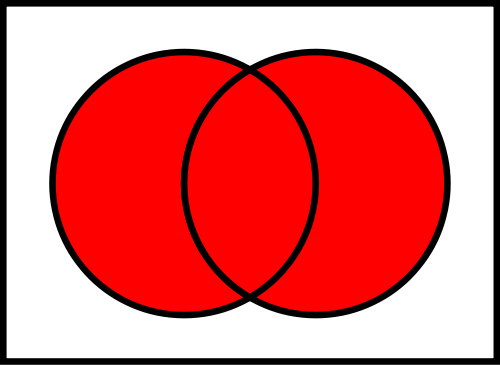
\includegraphics[scale=0.25]{AcupB}\label{fig:union}}
\subfigure[Intersection]{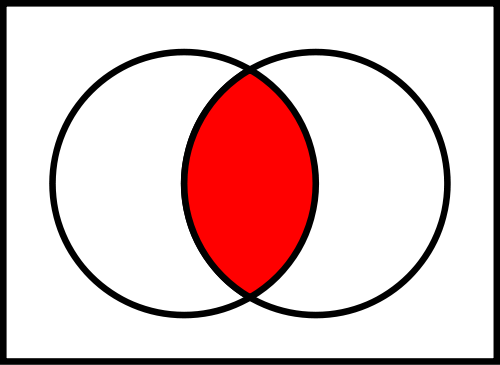
\includegraphics[scale=0.25]{AcapB}\label{fig:intersection}}
\subfigure[Complement]{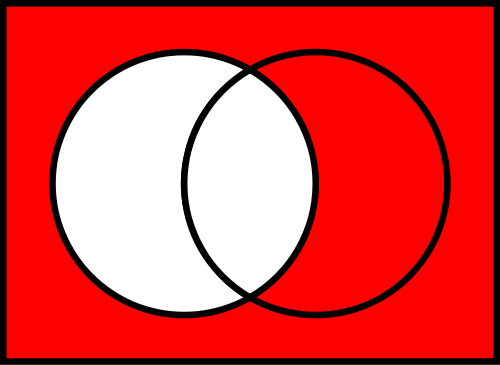
\includegraphics[scale=0.25]{Acomp}\label{fig:complement}}
\caption{Three figures using \texttt{subfigure}.\label{fig:setops-subfig}}
\end{figure}


Goodbye
\end{document}